%% lic_prac.tex
%%
%% Presentation of the course ``Legal Issues'' of the Official Master on Libre Software (URJC)
%% http://master.libresoft.es
%%


%%---------------------------------------------------------------------
%%---------------------------------------------------------------------

\begin{frame}
  \frametitle{Course Contents}

  \begin{itemize}
    \item Lesson 0: Presentation of the Course
    \item Lesson 1: Intellectual Property: basic concepts and legal framework
    \item Lesson 2: Legal Aspects of Libre Software
    \item Lesson 3: Libre software licenses
    \item Lesson 4: Free licenses for other intellectual works
    \item \alert{Lesson 5: Case studies}
  \end{itemize}

\end{frame}

%%%%%%%%%%%%%%%%%%%%%%%%%%%%%%%%%%%%%%%%%%%%%%%%%%%%%%%%%%%%%%%%%%%%%%%
\section{Lesson V: Practical Issues. Case studies}
%%%%%%%%%%%%%%%%%%%%%%%%%%%%%%%%%%%%%%%%%%%%%%%%%%%%%%%%%%%%%%%%%%%%%%%

%%%%%%%%%%%%%%%%%%%%%%%%%%%%%%%%%%%%%%%%%%%%%%%%%%%%%%%%%%%%%%%%%%%%%%%

\begin{frame}
\frametitle{Choosing a free license: previous criteria}

\begin{itemize}
\item Each project has its own goals and criteria related to licensing issues.
\item The main criteria of differentiation is existence (or not) of \alert{reciprocity pacts}.
\item Other copyleft licenses have a limited effect, which applies only to the work (or component) original (weak copyleft). 
\item Dual licensing policies.

\end{itemize}

\end{frame}

%%%%%%%%%%%%%%%%%%%%%%%%%%%%%%%%%%%%%%%%%%%%%%%%%%%%%%%%%%%%%%%%%%%%%%%

\begin{frame}
\frametitle{Choosing a free license: When?}

\begin{itemize}
\item When we want to guarantee some basic freedoms, common to all free software.
\item When we want a work achieves the highest use and dissemination (permissive licenses).
\item When we want to maintain control over the evolution of the program (copyleft licenses).
\item When we impose certain conditions or restrictions (the recognition of authorship, lack of liability, extra warranties, trademarks, etc.)
\end{itemize}

\end{frame}

%%%%%%%%%%%%%%%%%%%%%%%%%%%%%%%%%%%%%%%%%%%%%%%%%%%%%%%%%%%%%%%%%%%%%%%

\begin{frame}
\frametitle{How to know when a software license is free?}

\begin{center}
\includegraphics[width=6.5cm]{figs/chart.jpg}
\end{center}

\end{frame}

%%%%%%%%%%%%%%%%%%%%%%%%%%%%%%%%%%%%%%%%%%%%%%%%%%%%%%%%%%%%%%%%%%%%%%%

\begin{frame}
\frametitle{How to know when a software license is free?}

\begin{center}
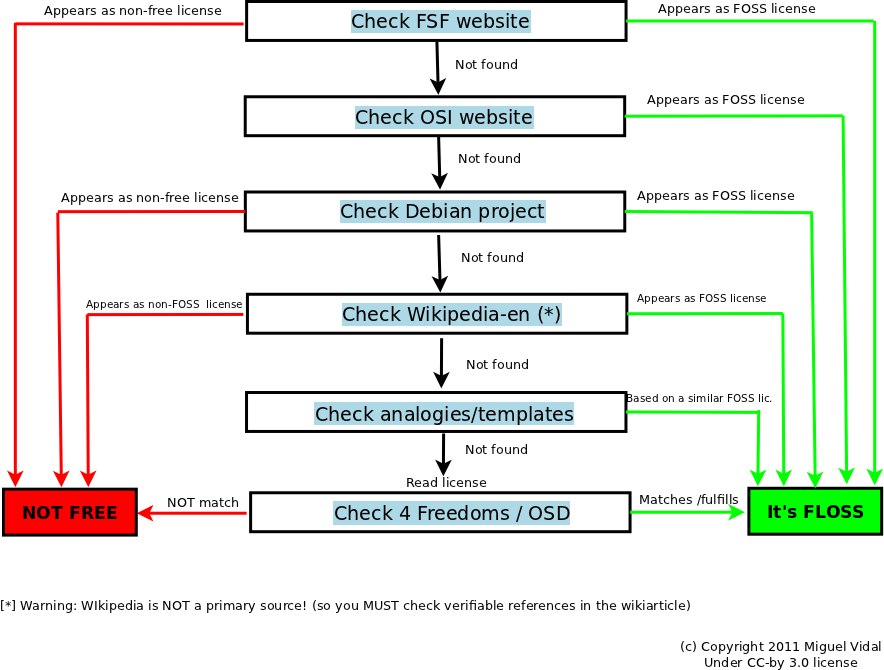
\includegraphics[width=10cm]{figs/flowchart-licenses.png}
\end{center}

\end{frame}


%%%%%%%%%%%%%%%%%%%%%%%%%%%%%%%%%%%%%%%%%%%%%%%%%%%%%%%%%%%%%%%%%%%%%%%

\begin{frame}
\frametitle{Choosing a free license: Cases}

\begin{itemize}
\item Do I want to allow privatization of derivative works?
\pause
\item Do I want developers return their modifications to the community, or me as original author, in particular?
\pause
\item Do I want to allow licensees to merge or link their program with mine?
\pause
\item Do I want widespread coverage and/or try to establish a standard?
\pause
\item Should my program run with one in particular? Have it any restrictions?
\pause
\item Is there risk that someone requiring a patent license over program?
\end{itemize}


\end{frame}

%%%%%%%%%%%%%%%%%%%%%%%%%%%%%%%%%%%%%%%%%%%%%%%%%%%%%%%%%%%%%%%%%%%%%%%

\begin{frame}
\frametitle{Quick Reference For Choosing a Free Software License}

\begin{center}
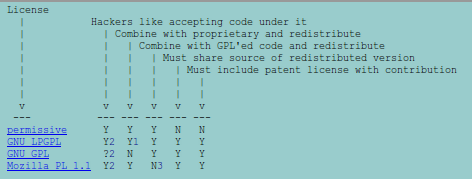
\includegraphics[width=11.5cm]{figs/licenses_quick_reference.png}
\end{center}

\end{frame}

%%%%%%%%%%%%%%%%%%%%%%%%%%%%%%%%%%%%%%%%%%%%%%%%%%%%%%%%%%%%%%%%%%%%%%%

\begin{frame}
\frametitle{Exercise: Find mistakes}

\begin{center}
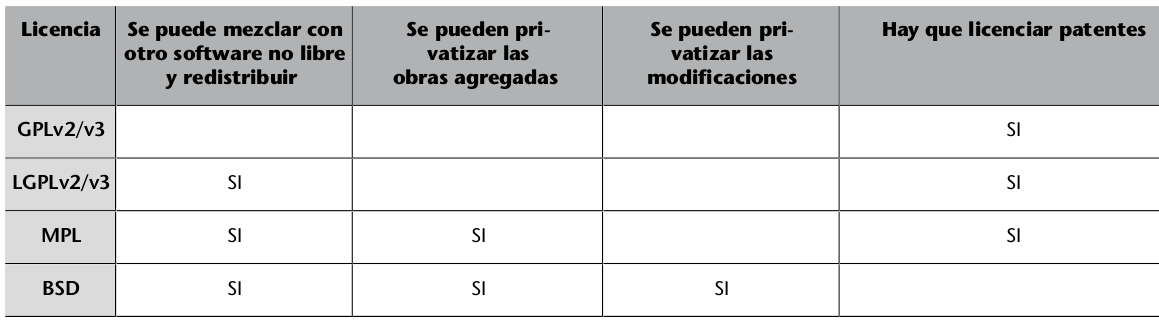
\includegraphics[width=11.5cm]{figs/tabla_licencias.png}
\end{center}

\end{frame}

%%%%%%%%%%%%%%%%%%%%%%%%%%%%%%%%%%%%%%%%%%%%%%%%%%%%%%%%%%%%%%%%%%%%%%%

\begin{frame}
\frametitle{Conventional Matrix}

\begin{center}
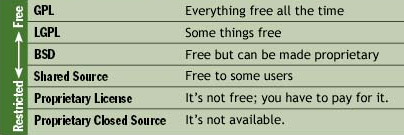
\includegraphics[width=11.5cm]{figs/conventional_matrix.png}
\end{center}

\end{frame}

%%%%%%%%%%%%%%%%%%%%%%%%%%%%%%%%%%%%%%%%%%%%%%%%%%%%%%%%%%%%%%%%%%%%%%%

\begin{frame}
\frametitle{Matrix Including Developer's Choice}

\begin{center}
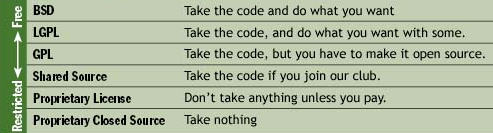
\includegraphics[width=11.5cm]{figs/matrix_developers_choice.png}
\end{center}

\end{frame}


%%%%%%%%%%%%%%%%%%%%%%%%%%%%%%%%%%%%%%%%%%%%%%%%%%%%%%%%%%%%%%%%%%%%%%%

\begin{frame}
\frametitle{Remarks}

\begin{itemize}
\item Some members of the community refuse to accept GPL'ed source code into their projects.
\item Other members of the community strongly prefer GPL'ed source code over other licenses.
\item Nobody refuses to accept code under permissive licenses such as BSD, X11, MIT... 
\end{itemize}

\end{frame}

%%%%%%%%%%%%%%%%%%%%%%%%%%%%%%%%%%%%%%%%%%%%%%%%%%%%%%%%%%%%%%%%%%%%%%%

\begin{frame}
\frametitle{Remarks (2)}

\begin{itemize}
\item Almost nobody refuses to accept LGPL'ed code, except the Apache Foundation, saying that they think it would impose LGPL requirement upon the proprietary code (when they are linked via the Java class-loading mechanism).
\item The FSF disagrees with this statement, asserting that such linking falls under section 6 of the LGPLv2 (linking exception).
\end{itemize}

\end{frame}

%%%%%%%%%%%%%%%%%%%%%%%%%%%%%%%%%%%%%%%%%%%%%%%%%%%%%%%%%%%%%%%%%%%%%%%

\begin{frame}
\frametitle{Remarks (and 3)}

\begin{itemize}
\item MPL 1.1 can be specifically amended to allow combining with GPL (section 13).
\item You should also get your employer (if you work as a programmer) or school, to sign a ``copyright disclaimer'' for the program, if necessary. 
\end{itemize}

\end{frame}


%%%%%%%%%%%%%%%%%%%%%%%%%%%%%%%%%%%%%%%%%%%%%%%%%%%%%%%%%%%%%%%%%%%%%%%

\begin{frame}
\frametitle{Applying a free license}


\begin{itemize}
\item \texttt{LICENSE} or \texttt{COPYING} file.
\item Copyright and license summary at the beginning of each source file.
\item It should have at least the ``copyright'' notice and a link to the full version of the license.
\item Also add information on how to contact you by electronic and paper mail.
\item If the program is interactive (terminal), make it output a short copyright notice 
when it starts in an interactive mode.
\item If it has a GUI, a menu can include copyright notice (or even the full license).
\end{itemize}

\end{frame}

%%%%%%%%%%%%%%%%%%%%%%%%%%%%%%%%%%%%%%%%%%%%%%%%%%%%%%%%%%%%%%%%%%%%%%%

\begin{frame}
\frametitle{Example: How to Apply the GPL to Your Work}

\footnotesize

\texttt{<one line with program's name and a brief idea of what it does.>} \\
\texttt{Copyright (C) <year>  <name of author>}

\medskip

\texttt{This program is free software: you can redistribute it and/or modify
    it under the terms of the GNU General Public License as published by
    the Free Software Foundation, either version 3 of the License, or
    (at your option) any later version.}

\medskip

\texttt{This program is distributed in the hope that it will be useful,
    but WITHOUT ANY WARRANTY; without even the implied warranty of
    MERCHANTABILITY or FITNESS FOR A PARTICULAR PURPOSE.  See the
    GNU General Public License for more details.}

\medskip

\texttt{You should have received a copy of the GNU General Public License
    along with this program.  If not, see <http://www.gnu.org/licenses/>.}


\end{frame}

%%%%%%%%%%%%%%%%%%%%%%%%%%%%%%%%%%%%%%%%%%%%%%%%%%%%%%%%%%%%%%%%%%%%%%%

\begin{frame}
\frametitle{Example: How to Apply the Apache License to Your Work}

\footnotesize

\texttt{Copyright [yyyy] [name of copyright owner]}

\medskip

\texttt{Licensed under the Apache License, Version 2.0 (the ``License'');
   you may not use this file except in compliance with the License.
   You may obtain a copy of the License at http://www.apache.org/licenses/LICENSE-2.0}

\medskip

\texttt{Unless required by applicable law or agreed to in writing, software
   distributed under the License is distributed on an ``AS IS'' BASIS,
   WITHOUT WARRANTIES OR CONDITIONS OF ANY KIND, either express or implied.
   See the License for the specific language governing permissions and
   limitations under the License.}


\end{frame}

%%%%%%%%%%%%%%%%%%%%%%%%%%%%%%%%%%%%%%%%%%%%%%%%%%%%%%%%%%%%%%%%%%%%%%%

\begin{frame}
\frametitle{Example: How to Apply the ISC License to Your Work (1)}

\begin{itemize}
\item Below is an example license to be used for new code in OpenBSD,
modeled after the ISC license.
\item It is important to specify the year of the copyright.  Additional years
should be separated by a comma, e.g.
    Copyright (c) 2003, 2004
\item If you add extra text to the body of the license, be careful not to
add further restrictions.
\end{itemize}

\end{frame}

%%%%%%%%%%%%%%%%%%%%%%%%%%%%%%%%%%%%%%%%%%%%%%%%%%%%%%%%%%%%%%%%%%%%%%%

\begin{frame}
% \frametitle{Example: How to Apply the ISC License to Your Work (and 2)}

\begin{block}{Example: How to Apply the ISC License to Your Work}
\footnotesize
/* \\
 * Copyright (c) CCYY YOUR NAME HERE $<$user@your.dom.ain$>$ \\
 * \\
 * Permission to use, copy, modify, and distribute this software \\
 * for any purpose with or without fee is hereby granted, provided \\
 * that the above copyright notice and this permission notice appear \\
 * in all copies. \\
 * \\
 * THE SOFTWARE IS PROVIDED "AS IS" AND THE AUTHOR DISCLAIMS \\
 * ALL WARRANTIES WITH REGARD TO THIS SOFTWARE INCLUDING \\
 * ALL IMPLIED WARRANTIES OF MERCHANTABILITY AND FITNESS. \\
 * IN NO EVENT SHALL THE AUTHOR BE LIABLE FOR ANY SPECIAL, \\
 * DIRECT, INDIRECT, OR CONSEQUENTIAL DAMAGES OR ANY \\
 * DAMAGES WHATSOEVER RESULTING FROM LOSS OF USE, DATA OR \\
 * PROFITS, WHETHER IN AN ACTION OF CONTRACT, NEGLIGENCE OR \\
 * OTHER TORTIOUS ACTION, ARISING OUT OF OR IN CONNECTION \\
 * WITH THE USE OR PERFORMANCE OF THIS SOFTWARE. \\
 */
\end{block}

\end{frame}



%%%%%%%%%%%%%%%%%%%%%%%%%%%%%%%%%%%%%%%%%%%%%%%%%%%%%%%%%%%%%%%%%%%%%%%
\begin{frame}
\frametitle{Dual-licensing}

Distribute software under two different sets of terms and conditions. Motivations:

\begin{itemize}
\item License compatibility (Perl, Mozilla/Firefox, MySQL).
\item Market segregation based business models (MySQL Enterprise)
\item Allows the holder to offer customisations, early releases, generate other derivative works or grant rights to third parties to redistribute proprietary versions.
\end{itemize}

                                                 
\end{frame}


%%%%%%%%%%%%%%%%%%%%%%%%%%%%%%%%%%%%%%%%%%%%%%%%%%%%%%%%%%%%%%%%%%%%%%%

\begin{frame}
\frametitle{Compatibility}

\begin{itemize}
\item Two licenses are incompatible if it is not possible combining both works in compliance with the terms of  both licenses at the same time. 
\item It affects to distribution, not the use. 
\item If two licenses are free does, it doesn't imply are compatible. 
\item Copyleft licenses are mutually incompatible, unless compatibility is declared explicitly. 
\item Support for `` linking'': even if not allowed mix or integrate software with different licenses, maybe it can be linked. 
\end{itemize}

\end{frame}

%%%%%%%%%%%%%%%%%%%%%%%%%%%%%%%%%%%%%%%%%%%%%%%%%%%%%%%%%%%%%%%%%%%%%%%

\begin{frame}
\frametitle{Forking (1)}

\begin{itemize}
\item A piece of software is modified and developed separately by another team development, and distributed under a different name, and maybe other
license.
\item The forks can be possible \alert{only} with free/open source software.
\item The GPL software has tendency to avoid forking (we must keep the original license).
\item The BSD-style licenses are forked easily.
\end{itemize}

\end{frame}

%%%%%%%%%%%%%%%%%%%%%%%%%%%%%%%%%%%%%%%%%%%%%%%%%%%%%%%%%%%%%%%%%%%%%%%

\begin{frame}
\frametitle{Forking (and 2)}

\begin{itemize}
\item Forking is considered a bad thing (waste efforts, bitter disputes...).
\item But there are successful cases: XOrg/XFree86, 386BSD, OpenBSD, Gnu-Emacs/XEmacs, changes of license (GForge, OpenSSH).
\end{itemize}

\end{frame}


%%%%%%%%%%%%%%%%%%%%%%%%%%%%%%%%%%%%%%%%%%%%%%%%%%%%%%%%%%%%%%%%%%%%%%%

\begin{frame}
\frametitle{Licenses and warranty}

\begin{itemize}
\item Warranty disclaimers and limitation of liability clauses are common in software.
\item There are legal doubts about the effectiveness of these clauses: \alert{would not apply to consumers}.
\item This clauses are valid when there is \alert{no commercial service}.
\item The proprietary licenses using similar terms: is a myth to accept greater responsibility.
\item It must be considered legal guarantees that apply to both open source and proprietary software.
\item The free licenses allow (sometimes) to add extra warranty clauses.
\end{itemize}


\end{frame}

%%%%%%%%%%%%%%%%%%%%%%%%%%%%%%%%%%%%%%%%%%%%%%%%%%%%%%%%%%%%%%%%%%%%%%%

\begin{frame}
\frametitle{Exercise: Case study}


\begin{itemize}
\item Case study: Apache License v2 and GPL (v2 and v3)  (in)compatibility.
\item Moodle exercise.
\end{itemize}

\end{frame}


%%%%%%%%%%%%%%%%%%%%%%%%%%%%%%%%%%%%%%%%%%%%%%%%%%%%%%%%%%%%%%%%%%%%%%%

\begin{frame}
\frametitle{Exercise: Case study}


\begin{itemize}
\item Case study: GPL and CDDL incompatibility. 
\item Moodle exercise.
\end{itemize}

\end{frame}


%%%%%%%%%%%%%%%%%%%%%%%%%%%%%%%%%%%%%%%%%%%%%%%%%%%%%%%%%%%%%%%%%%%%%%%

\begin{frame}
\frametitle{Exercise: Case study}


\begin{itemize}
\item Case study: The EUPL
\item Moodle Exercise 
\end{itemize}

\end{frame}


%%==================================================================
%%---------------------------------------------------------------


